%
% nullstellen.tex
%
% (c) 2020 Prof Dr Andreas Müller, Hochschule Rapperswil
%
\section{Nullstellen von Funktionen
\label{buch:section:nullstellen}}
\rhead{Nullstellen von Funktionen}
Die Aufgabe, eine Gleichung der Form $f(x) = g(x)$
zu lösen, also ein $x\in\mathbb R$ zu finden derart, dass die Gleichung
erfüllt wird, ist gleichbedeutend damit, eine Nullstelle der Funktion
$f(x)-g(x)$ zu finden.
Es ist also gar nicht nötig, allgemeine Gleichungslösungsverfahren zu
entwickeln, es reicht völlig aus, Nullstellen finden zu können.

Es muss davon ausgegangen werden, dass die Funktion $f$ nicht einfach
algebraisch invertiert werden kann.
Sie wird also als Black-Box behandelt, man kann mit ihr nur Funktionswerte
zu vorgegebenen $x$ ermitteln.
Bei einem Versuch mit einem Wert $x_0$ gibt der Funktionswert $f(x_0)$
nur die Information, ob der Versuch erfolgreich war oder nicht.
Grundsätzlich können wir nicht einmal schliessen, dass ein
grosser Funktionswert bedeutet, dass $x_0$ weit von einer
Nullestelle entfernt liegt.
Dazu sind weitere Annahmen über die Funktion notwendig.

In diesem Abschnitt untersuchen wir, wie verschiedene ergänzende Annahmen
über die Funktion $f$ die Möglichkeiten erweitern, Nullstellen
effizient zu finden.
In keinem Fall werden wir allerdings Differenzierbarkeit von $f$ voraussetzen,
dies ist Abschnitt~\ref{buch:section:newtion} vorbehalten, wo das
Newton-Verfahren behandelt wird..

%
% Intervallhalbierung
%
\subsection{Intervallhalbierung
\label{buch:subsection:intervallhalbierung}}
Ist die Funktion stetig, sagt die Grösse eines Funktionswertes immer
noch nichts darüber aus, wie weit das Argument von der Nullstelle
entfernt ist.
Zwei Werte mit unterschiedlichem Vorzeichen zeigen dagegen klar an,
dass sich eine Nullstellen zwischen Argumenten befinden muss.
Dies ist der Inhalt des folgenden Spezialfalls des Zwischenwertsatzes.

\begin{satz}[Zwischenwertsatz für Nullstellen]
\label{buch:satz:nullstellenzwsatz}
Ist die Funktion $f\colon[a,b]\to\mathbb R$ stetig mit $f(a) <0$ und $f(b)>0$,
dann hat $f$ eine Nullstelle im Inneren des Intervals $[a,b]$.
\end{satz}

\begin{figure}
\centering
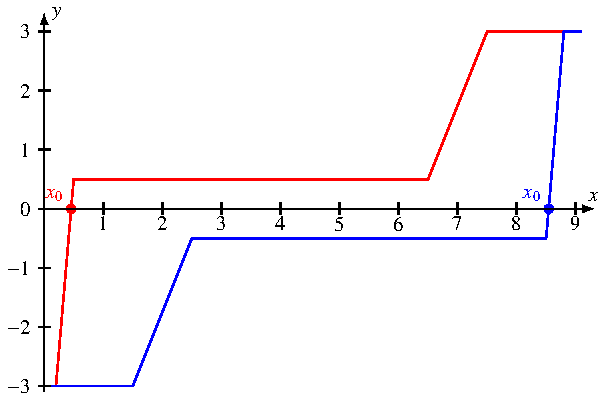
\includegraphics{chapters/20-gleichungen/figures/stufe.pdf}
\caption{Die Werte einer stetigen Funktion an den Intervallenden verraten
nichts über die Lage einer Nullstelle im Interval.
Die beiden Graphen gehören zu Funktionen, die den gleichen Wert an den
Intervallenden haben, aber die Nullstelle $x_0$ liegt an völlig
unterschiedlichen Stellen
\label{buch:figure:stufe}}
\end{figure}

Man beachte, dass der Betrag der Funktionswerte an den Intervallenden keine
Information darüber liefert, wo im Interval die Nullstelle zu finden ist.
Abbildung~\ref{buch:figure:stufe} zeigt zwei Funktionen mit identischen
Funktionswerten an den Intervallenden aber völlig verschiedener Lage
der Nullstellen.
Erst zusätzliche Annahmen über die Steigung oder Krümmung der Kurve können
die Lage der Nullstelle besser eingrenzen.

Der Zwischenwertsatz~\ref{buch:satz:nullstellenzwsatz} liefert trotzdem
genug Information, um die Nullstelle zu finden.
Für die folgende Diskussion nehmen wir der Einfachheit an, dass $f(a)<0$
und $f(b)>0$ ist.
Wir wissen bereits, dass die Nullstelle im Interval $[a,b]$ liegen muss.
Sei $m=\frac12(a+b)$ der Mittelpunkt des Intervals.
Wenn $f(m) > 0$ ist, können wir schliessen, dass eine Nullstelle im
Teilinterval $[a,m]$ liegen muss.
Wenn $f(m) <0$ ist, liegt eine Nullstelle in $[m,b]$.
Damit ist ein neues Interval halber Länge gefunden, welches eine
Nullstelle von $f$ enthält.
Wir haben ein Bit Information über die Nullstelle gewonnen.
Durch Wiederholen dieses Prozesses können wir ein beliebige kleines
Interval erhalten, welches eine Nullstelle enthält.
Nach dem Intervalschachtelungsprinzip der Analysis definiert dies
die Nullstelle.

\begin{satz}[Intervallhalbierung]
Sei $f\colon[a,b]\to\mathbb R$ eine stetige Funktion mit $f(a)<0$ und
$f(b)>0$.
Sei $I_k=[a_k,b_k]$ die Folge von Intervallen rekursiv definiert wie folgt.
\begin{enumerate}
\item
Das Startinterval hat Intervallenden $a_0=a$ und $b_0=b$.
\item
Sei $m_k = \frac12(a_k+b_k)$.
Das Intervall $I_{k+1}$ ist 
\[
I_{k+1} = [a_{k+1},b_{k+1}] = 
\begin{cases}
[a_k,m_k]&\qquad f(m_k) > 0\\[5pt]
[m_k,b_k]&\qquad f(m_k) < 0.
\end{cases}
\]
\end{enumerate}
Die Intervalle $I_k$ haben die folgenden Eigenschaften
\begin{enumerate}
\item
Die Länge der Intervalle halbiert sich in jeder Iteration: $|I_k|=2^{-k}(b-a)$.
\item
Für jedes Intervall gilt $f(a_k)<0$ und $f(b_k)> 0$.
\item
Die Schnittmenge
$\bigcap_{k=0}^\infty I_k$ enthält nur den Wert
\begin{equation}
x_0 = \lim_{k\to\infty}a_k=\lim_{k\to\infty}b_k=\lim_{k\to\infty}m_k,
\label{buch:gleichungen:intervalkonvergenz}
\end{equation}
der eine Nullstelle der Funktion $f$ ist.
\end{enumerate}
\end{satz}

\begin{proof}[Beweis]
Es ist nur noch die Ausssage~\eqref{buch:gleichungen:intervalkonvergenz}
über die Konvergenz der Folgen $a_k$ und $b_k$
zu beweisen.
Da aber die Intervall-Länge $|I_k|=2^{-k}(b-a)$ ist, kann man die
Entfernung der Folgenglieder voneinander abschätzen.
Ist $k=\min\{m,n\}$, dann folgt
\[
|a_m-a_n| < 2^{-k}(b-a),\quad
|b_m-b_n| < 2^{-k}(b-a),\quad
|m_m-m_n| < 2^{-k}(b-a).
\]
Wählt man $N$ so gross, dass $2^{-N}(b-a)<\varepsilon$ ist, dann
folgt für jedes beliebige $\varepsilon>0$, dass 
\[
|a_m-a_n|<\varepsilon,\quad
|b_m-b_n|<\varepsilon,\quad
|m_m-m_n|<\varepsilon
\]
ist.
Die Folgen sind also Cauchy-Folgen.
\end{proof}

Die Konvergenzgeschwindigkeit des Intervall-Halbierungs-Verfahrens ist
sehr beschränkt.
Der Fehler halbiert sich in jeder Iteration, man gewinnt also genau
1 Bit Genauigkeit.
Für die volle Genauigkeit eines Gleitkomma-Typs der Maschine braucht
man also etwa soviele Iterationen, wie die Mantisse Binärstellen hat,
aber auch nur, wenn das erste Bit und der Exponent bereits richtig
sind.

\begin{beispiel}
Als Beispiel berechnen wir $\sqrt[100]{10}$.
Die Potenzfunktion $p(x)=x^{100}$, die wir dazu invertieren müssen, hat
extrem grosse Steigung in der Näher der Lösung.
Es muss eine Nullstelle der Funktion $f(x)=x^{100}-10$ gefunden werden.
Wegen $f(0)=-10$ und $f(2)\approx 1.2677\cdot 10^{30}$ muss das Intervall
$[0,2]$ eine Nullstelle enthalten.
Weil die Funktion monoton wachsend ist, ist es auch die einzige.
Der Wert $f(2)$ ist klein genug für den \texttt{float} Typ,
daher kann man die Berechnung in \texttt{float} durchführen.

\begin{table}
\centering
\begin{tabular}{|>{$}r<{$}|>{$}r<{$}|>{$}r<{$}|>{$}r<{$}|}
\hline
k&a_k&b_k& b_k-a_k\\
\hline
 0 & 0.00000000 & 2.00000000 & 2.00000000\\
  1 & \color{red} \underline{1}.00000000 &             \underline{}2.00000000 & 1.00000000\\
  2 &             \underline{1}.00000000 & \color{red} \underline{1}.50000000 & 0.50000000\\
  3 &             \underline{1}.00000000 & \color{red} \underline{1}.25000000 & 0.25000000\\
  4 &             \underline{1}.00000000 & \color{red} \underline{1}.12500000 & 0.12500000\\
  5 &             \underline{1}.00000000 & \color{red} \underline{1.0}6250000 & 0.06250000\\
  6 &             \underline{1}.00000000 & \color{red} \underline{1.0}3125000 & 0.03125000\\
  7 & \color{red} \underline{1.0}1562500 &             \underline{1.0}3125000 & 0.01562500\\
  8 &             \underline{1.0}1562500 & \color{red} \underline{1.023}43750 & 0.00781250\\
  9 & \color{red} \underline{1.0}1953125 &             \underline{1.023}43750 & 0.00390625\\
 10 & \color{red} \underline{1.02}148438 &             \underline{1.023}43750 & 0.00195312\\
 11 & \color{red} \underline{1.02}246094 &             \underline{1.023}43750 & 0.00097656\\
 12 & \color{red} \underline{1.02}294922 &             \underline{1.023}43750 & 0.00048828\\
 13 & \color{red} \underline{1.023}19336 &             \underline{1.023}43750 & 0.00024414\\
 14 &             \underline{1.023}19336 & \color{red} \underline{1.023}31543 & 0.00012207\\
 15 & \color{red} \underline{1.0232}5439 &             \underline{1.023}31543 & 0.00006104\\
 16 & \color{red} \underline{1.0232}8491 &             \underline{1.023}31543 & 0.00003052\\
 17 &             \underline{1.0232}8491 & \color{red} \underline{1.023}30017 & 0.00001526\\
 18 & \color{red} \underline{1.02329}254 &             \underline{1.023}30017 & 0.00000763\\
 19 &             \underline{1.02329}254 & \color{red} \underline{1.02329}636 & 0.00000381\\
 20 &             \underline{1.02329}254 & \color{red} \underline{1.02329}445 & 0.00000191\\
 21 &             \underline{1.02329}254 & \color{red} \underline{1.023293}50 & 0.00000095\\
 22 &             \underline{1.02329}254 & \color{red} \underline{1.023293}02 & 0.00000048\\
 23 & \color{red} \underline{1.02329}278 &             \underline{1.023293}02 & 0.00000024\\
 24 & \color{red} \underline{1.023292}90 &             \underline{1.023293}02 & 0.00000012\\
\hline
\end{tabular}
\caption{Bestimmung von $\sqrt[100]{10}$ mit Hilfe des
Intervallhalbierungsverfahrens.
Die jeweils neue Intervallgrenze ist {\color{red}rot} markiert.
\label{buch:table:intervallhalbierung}}
\end{table}

Tabelle~\ref{buch:table:intervallhalbierung} zeigt den Gang der
Berechnung.
Die Implementation in C++ verwendet als Abbruchkriterium die
Länge des Intervals.
Die Iteration endet, wenn 
die Intervallänge $b_k-a_k$ den $\varepsilon$-Wert
erreicht, der für den Typ \texttt{float} im Header
\texttt{limits} definiert ist.
Wie erwartet sind soviele Iterationen nötig, wie die Mantisse 
des \texttt{float}-Typs Bits hat.

Das Programm \texttt{nullstellen.cpp}\footnote{Das Programm
kann im Verzeichnis 
\texttt{buch/chapters/experiments/nullstellen} von \cite{buch:repo}
gefunden werden.}
implementiert den Algorithmus für jeden Maschinentypen.
Damit kann man sehen, dass die berechnete Laufzeit auch für die
grösseren Gleitkommatypen durch die Bitlänge der Mantisse gegeben ist.
\end{beispiel}

%
% Sekanten-Verfahren
%
\subsection{Sekanten-Verfahren
\label{buch:subsection:sekanten}}
Das Intervallhalbierungsverfahren verwendet nicht mehr als die
Stetigkeit der Funktion.
Dies führt zu sehr langsamer Konvergenz, weil die relative Grösse
der Funktionswerte in den Intervallenden keine Information über die
Lage der Nullstelle im Intervall gegen kann.
Dazu wird Information darüber benötigt, wie schnell sich Funktionswerte
ändern können.
Insbesondere muss davon ausgegangen werden können, dass die Steigung
der Funktion über das betrachtete Interval nicht zu stark schwankt.
Die Ableitung einer differenzierbaren Funktion kann diese Information
liefern, es ist aber ausreichend, eine Lipschitz-Bedingung zu verlangen,
die wie folgt definiert ist.

\begin{definition}
\label{buch:definition:lipshitz}
Die Funktion $f\colon[a,b]\to\mathbb R$ erfüllt eine Lipschitz-Bedingung
zum Exponenten $\alpha$, wenn es eine Konstante $L$ gibt derart, dass
\[
|f(x)-f(y)|
<
L|x-y|^\alpha
\]
ist.
\end{definition}

Eine Lipschitz-Bedingung begrenzt, wie schnell sich der Wert
einer Funktion ändern kann.
Eine stetig differenzierbare Funktion erfüllt automatisch eine
Lipschitz-Bedingung für $\alpha=1$, die Umkehrung gilt allerdings
nicht.

Sei jetzt $f\colon[a,b]\to\mathbb R$ wieder eine Funktion mit
$f(a)<0$ und $f(b) > 0$.
Wenn $f$ eine Lipschitz-Bedingung erfüllt, dann geben die
Werte $f(a)$ und $f(b)$ zusätzlich Information über die Lage
der Nullstelle, die im Interval liegen muss.
Da sich Funktionswerte nicht beliebig schnell ändern können,
dürfte die Nullstelle näher beim kleineren Funktionswert sein.

\begin{figure}
\centering
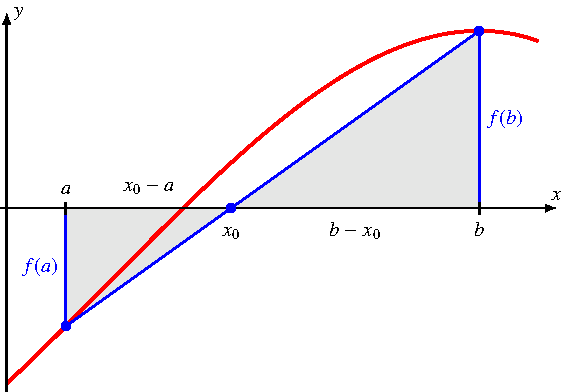
\includegraphics{chapters/20-gleichungen/figures/sekante.pdf}
\caption{Bestimmung einer neuen Schätzung $x_0$ für die Nullstelle
mit Hilfe der Sekante.
Nach dem Strahlensatz ist $(a-x_0):f(a) = (b-x_0):f(b)$, woraus
sich $x_0$ bestimmen lässt (siehe auch \eqref{buch:equation:sekante}).
\label{buch:figure:sekante}}
\end{figure}

Nehmen wir an, die Funktion $f$ sei linear zwischen den beiden
Funktionswerten, dann ist die Nullstelle der Schnittpunkt
der Geraden durch $(a,f(a))$ und $(b,f(b))$ mit der $x$-Achse
(Siehe auch Abildung~\ref{buch:figure:sekante}).
Der Strahlensatz zeigt
\[
\begin{aligned}
&&
(a-x_0) : f(a)
&=
(b - x_0) : f(b)
\\
&\Leftrightarrow&
a\,f(b) - b\,f(a)
&=
x_0(f(b)-f(a))
\\
&\Rightarrow&
x_0
&=
\frac{a\,f(b)-b\,f(a)}{f(b)-f(a)}.
\end{aligned}
\]
Man kann diese Formel für $x_0$ auch bekommen als mit den
Funktionswerten gewichtetes Mittel der Endpunkte wie folgt.
Das Gewicht $m_a$ von $a$ ist $f(b)$, das Gewicht $m_b$ von
$b$ ist $-f(a)$, hier verwenden wir $f(a)<0$.
Das gewichtete Mittel ist dann
\begin{equation}
\frac{a\,m_a+b\,m_b}{m_a+m_b}
=
\frac{a\,f(b)-b\,f(a)}{f(b)-f(a)}=x_0.
\label{buch:equation:sekante}
\end{equation}
Indem die Intervallhalbierung durch eine Teilung des
Intervalls im Punkt $x_0$ ersetzt wird, kann ein neuer Algorithmus
gewonnen werden, der möglicherweise schneller konvergiert, weil
Intervalle schneller kleiner werden können.
Allerdings deutet die Formel~\eqref{buch:equation:sekante} auf
ein weiteres Problem hin.
Ist der Nenner sehr klein, kann die neue Approximation $x_0$ weit
entfernt sein von $a$ und $b$.

Es ist leider auch nicht so, dass das neue Verfahren unbedingt schneller 
konvergiert.
Im Intervallhalbierungsverfahren ist sichergestellt, dass das neue
Intervall höchstens halb so gross ist.
Eine solche Garantie gibt es bei Verwendung der
Formel~\eqref{buch:equation:sekante} nicht.
Ist zum Beispiel im Interval $[a,b]$ die erste Ableitung $f'(x)>0$ und
die zweite Ableitung $f''(x)<0$,
dann ist der neue Teilpunkt immer rechts von der Nullstelle.
Das neue Intervall hat daher immer den gleichen linken Endpunkt $a$,
die Folge $a_k$ konvergiert nicht.

\begin{beispiel}
Die Funktion $f(x)=\sin x - \frac12$ hat im Interval $[0,\frac{\pi}2]$
positive Steigung und negative zweite Ableitung.
Wie erwartet bleibt $a_k$ konstant, aber $b_k$ konvergiert monton
gegen die Nullstelle.
In Tabelle~\ref{buch:table:sekanten} sind die Resultate der Rechnung
gezeigt.
Die Werte der Teilpunkte $m_k$ konvergiert linear gegen den gesuchten
Wert $\arcsin\frac12$.
\begin{table}
\centering
\begin{tabular}{|>{$}r<{$}|>{$}r<{$}|}
\hline
  k & m_k \\
\hline
 -1 & 0.00000000 \\
  0 & 1.50000000 \\
  2 & \underline{0.5}5041450 \\
  3 & \underline{0.52}616811 \\
  4 & \underline{0.523}83864 \\
  5 & \underline{0.5236}2108 \\
  6 & \underline{0.5236}0088 \\
  7 & \underline{0.523598}97 \\
  8 & \underline{0.523598}79 \\
\hline
\end{tabular}
\caption{Sekanten-Verfahren zur Bestimmung von $\arcsin \frac12$.
Die Konvergenz ist ungefähr linear, aber deutlich schneller als
beim Intervallhalbierungsverfahren.
\label{buch:table:sekanten}}
\end{table}
\end{beispiel}

Ein gut konvergentes Verfahren kann man also nur erwarten, wenn man
sicherstellen kann, dass sich die Funktion im Intervall merklich
ändert, dass als $f(x)-f(y)$ nicht zu klein wird.
Dies wird erreicht, wenn $f$ eine {\em untere Lipschitz-Bedingung}
erfüllt.
Dies bedeutet, dass es eine Zahl $l>0$ gibt derart, dass
\[
|f(x)-f(y)| \ge l\cdot |x-y|^\alpha.
\]
\index{Lipschitz-Bedingung!untere}%
\index{untere Lipschitz-Bedingung}%
Solche Lipschitz-Bedingungen sind automatisch erfüllt, wenn eine 
Funktion stetig differenzierbar ist, dies ist auch für die Praxis der
übliche Fall.

\begin{satz}[Sekanten-Verfahren]
Sei $f\colon[a,b]\to\mathbb R$ eine stetig differenzierbare Funktion mit
$f(a)<0$ und $f(b)>0$.
Man setzt $x_{-1}=a$ und $x_0=b$ und konstruiert die Folge
\begin{equation}
x_{n+1} = \frac{x_{n-1}f(x_n) - x_nf(x_{n-1})}{f(x_{n})-f(x_{n-1})}.
\label{buch:eqn:sekanten-iteration}
\end{equation}
Falls $a$ und $b$ nahe genug bei einer Nullstelle der Funktion $f$ ist,
dann konvergiert die Folge $x_{n+1}$ gegen die Nullstelle.
\end{satz}

\begin{proof}[Beweis]
Sie $\bar{x}$ die gesuchte Nullstelle im Intervall $[a,b]$.
Da wir andernfalls $f(x)$ durch $-f(x)$ ersetzen können, können wir
ohne Beschränkung der Allgemeinheit annehmen, dass $f(a)<0$
und $f(b)>0$ gilt.
Es gibt dann Zahlen $l$ und $L$ derart, dass
\[
l\cdot |x-y|
<
|f(x)-f(y)|
<
L\cdot |x-y|
\]
für Argumente $x$ und $y$ in einer Umgebung von $\bar{x}$.

XXX TODO
\end{proof}

Die Iterationsformel \eqref{buch:eqn:sekanten-iteration} hat den
gravierenden Nachteil, dass in der Nähe der Lösung die beiden
Grössen im Zähler und im Nenner fast gleich gross sind und damit
starke Auslöschung auftreten wird.
Die Umformung
\begin{align}
x_{n+1}
&=
\frac{x_{n-1}f(x_{n})-x_{n}f(x_{n-1})}{f(x_n)-f(x_{n-1})}
=
\frac{x_{n-1}f(x_{n})
{\color{red}\mathstrut -x_{n-1}f(x_{n-1})+x_{n-1}f(x_{n-1})}
-x_{n}f(x_{n-1})}{f(x_n)-f(x_{n-1})}
\\
&=x_{n-1} - f(x_{n-1})\frac{x_n-x_{n-1}}{f(x_n)-f(x_{n-1})}
\label{buch:sekante:stabil}
\end{align}
ist algebraisch identisch, jedoch wird in der letzten Form die Approximation
$x_{n-1}$ um einen Betrag korrigiert, der umso kleiner wird, je besser
$x_{n-1}$ die Nullstelle bereits approximiert und damit je kleiner
der Faktor $f(x_{n-1})$ ist.
Der Bruch in \eqref{buch:sekante:stabil} kann jedoch immer noch
erratische Werte annehmen und damit die Konvergenz des Verfahrens
gefährden.

Man beachte, dass die Bedingung an die Vorzeichen von $f(a)$ und $f(b)$
nur dazu dient, die Existenz einer Nullstelle im Intervall zu garantieren.
Ein anderes Problem dieses Verfahrens ist, dass mit genauer werdender
Approximation $x_n$ der Nullstelle die Werte $f(x_n)$ und $f(x_{n-1})$
sehr nahe beeinander liegen und damit die Differenz stark von 
Auslöschung betroffen sein wird.
Im Intervallhalbierungsalgorithmus ist dies kein Problem, weil keine
Differenzen von Funktionswerten gebildet werden und ausschliesslich das
Vorzeichen des Funktionswertes verwendet wird, die Genauigkeit hat
keinen Einfluss auf das Vorzeichen.



